\documentclass[aspectratio=169,11pt]{beamer}

\usetheme{default}
\usefonttheme{professionalfonts}
\setbeamertemplate{navigation symbols}{}
\setbeamertemplate{footline}{}
\setbeamertemplate{headline}{}

\usepackage[T1]{fontenc}
\usepackage{lmodern}
\usepackage{tikz}
\usepackage{graphicx}
\usepackage{listings}
\usepackage{array}
\usepackage{booktabs}
\usepackage{ragged2e}
\usetikzlibrary{arrows.meta,positioning,calc,shapes.geometric,fit}

\definecolor{Paper}{HTML}{FFF7ED}
\definecolor{PaperSoft}{HTML}{FFFDF8}
\definecolor{Ink}{HTML}{221714}
\definecolor{Muted}{HTML}{6B5A50}
\definecolor{Line}{HTML}{E7CDB7}
\definecolor{Coral}{HTML}{EF5B42}
\definecolor{Blue}{HTML}{2F8CEB}
\definecolor{Gold}{HTML}{F5B842}
\definecolor{Green}{HTML}{2E9C6D}
\definecolor{Red}{HTML}{C44536}
\definecolor{Navy}{HTML}{10233F}

\setbeamercolor{background canvas}{bg=Paper}
\setbeamercolor{normal text}{fg=Ink}
\setbeamercolor{frametitle}{fg=Ink}
\setbeamercolor{structure}{fg=Coral}

\newcommand{\decktitle}[1]{%
  {\fontsize{31}{34}\selectfont\bfseries #1\par}
}
\newcommand{\decksubtitle}[1]{%
  \vspace{0.2cm}{\fontsize{13}{17}\selectfont\color{Muted}#1\par}
}
\newcommand{\slidetitle}[1]{%
  {\fontsize{25}{29}\selectfont\bfseries #1\par}
}
\newcommand{\smalllabel}[1]{%
  {\fontsize{8}{10}\selectfont\bfseries\color{Coral}\MakeUppercase{#1}\par}
}
\newcommand{\bigstat}[2]{%
  \begin{minipage}{0.44\linewidth}
    {\fontsize{30}{32}\selectfont\bfseries #1\par}
    {\fontsize{9}{12}\selectfont\color{Muted}#2\par}
  \end{minipage}
}
\newcommand{\plainitem}[1]{%
  \par\noindent\begin{tikzpicture}[baseline=-0.5ex]
    \fill[Coral] (0,0) circle (0.055);
  \end{tikzpicture}\hspace{0.35em}#1
}
\newcommand{\statuspill}[2]{%
  \tikz[baseline=-0.65ex]\node[rounded corners=5pt,draw=#1!55,fill=#1!12,inner xsep=6pt,inner ysep=3pt] {\scriptsize\bfseries #2};
}
\newcommand{\circicon}[2]{%
  \tikz[baseline=-0.7ex]\node[circle,draw=#1!55,fill=#1!12,minimum size=0.62cm,inner sep=0pt] {\scriptsize\bfseries #2};
}

\lstdefinestyle{code}{
  basicstyle=\ttfamily\scriptsize,
  keywordstyle=\color{Blue}\bfseries,
  stringstyle=\color{Green!70!black},
  commentstyle=\color{Muted},
  showstringspaces=false,
  frame=single,
  rulecolor=\color{Line},
  backgroundcolor=\color{PaperSoft},
  framerule=0.6pt,
  xleftmargin=0.2cm,
  xrightmargin=0.2cm,
  aboveskip=0.2cm,
  belowskip=0.2cm
}
\lstset{style=code}

\tikzset{
  nodebox/.style={draw=Line,fill=PaperSoft,rounded corners=8pt,minimum height=0.86cm,align=center,font=\scriptsize\bfseries,text=Ink,inner xsep=8pt},
  actionbox/.style={draw=Coral!45,fill=Coral!8,rounded corners=8pt,minimum height=0.86cm,align=center,font=\scriptsize\bfseries,text=Ink,inner xsep=8pt},
  storebox/.style={draw=Blue!45,fill=Blue!8,cylinder,shape border rotate=90,aspect=0.22,minimum height=0.9cm,minimum width=1.3cm,align=center,font=\scriptsize\bfseries,text=Ink},
  line/.style={-{Stealth[length=2.2mm]},draw=Muted!75,line width=0.75pt},
  softline/.style={-{Stealth[length=2.0mm]},draw=Line!90,line width=0.65pt}
}

\newenvironment{contentframe}[1]{%
  \begin{frame}[plain]
  \vspace{0.2cm}
  \slidetitle{#1}
  \vspace{0.32cm}
}{%
  \end{frame}
}

\begin{document}

\begin{frame}[plain]
\begin{tikzpicture}[remember picture,overlay]
  \fill[Paper] (current page.south west) rectangle (current page.north east);
  \node[anchor=east,opacity=0.96] at ([xshift=0.9cm,yshift=-0.05cm]current page.east)
    {
\includegraphics[height=8.1cm]{assets/fleeting-circus-hero.png}};
  \fill[Paper,opacity=0.72] (current page.south west) rectangle ([xshift=2.7cm]current page.north);
\end{tikzpicture}
\vspace{1.2cm}
\hspace{0.4cm}
\begin{minipage}{0.55\linewidth}
  \smalllabel{Bachelor project prototype}
  \decktitle{Fleeting Circus}
  \decksubtitle{A lightweight serverless platform for Python functions}
  \vspace{0.45cm}
  {\large Upload code. Build once. Invoke through an API.}
\end{minipage}
\end{frame}

\begin{contentframe}{The basic idea}
\centering
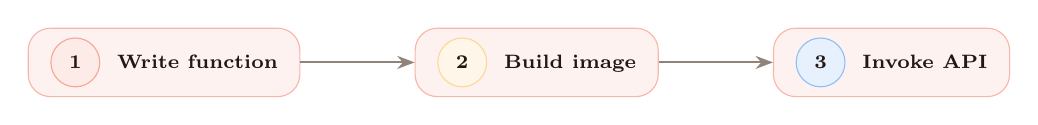
\begin{tikzpicture}[node distance=1.45cm]
  \node[actionbox,minimum width=2.8cm] (write) {\circicon{Coral}{1} Write function};
  \node[actionbox,minimum width=2.8cm,right=of write] (build) {\circicon{Gold}{2} Build image};
  \node[actionbox,minimum width=2.8cm,right=of build] (invoke) {\circicon{Blue}{3} Invoke API};
  \draw[line] (write) -- (build);
  \draw[line] (build) -- (invoke);
\end{tikzpicture}
\vspace{0.65cm}

{\Large Users bring Python code. The platform handles execution.}
\end{contentframe}

\begin{contentframe}{Why this project}
\begin{columns}[T,totalwidth=\linewidth]
  \begin{column}{0.50\linewidth}
    \Large
    \plainitem{No manual server setup}\par\vspace{0.35cm}
    \plainitem{Repeatable function builds}\par\vspace{0.35cm}
    \plainitem{API calls for execution}\par\vspace{0.35cm}
    \plainitem{Results and artifacts tracked}
  \end{column}
  \begin{column}{0.44\linewidth}
    
\begin{tikzpicture}
      \node[nodebox,minimum width=4.6cm,minimum height=3.4cm] (box) {};
      \node[align=center] at (box.center) {\fontsize{32}{34}\selectfont\bfseries code\\[0.15cm]\fontsize{17}{20}\selectfont in\\[0.15cm]\fontsize{32}{34}\selectfont\bfseries result};
      \draw[Coral,line width=1.3pt] ([xshift=-1.7cm,yshift=1.1cm]box.center) -- ([xshift=1.7cm,yshift=1.1cm]box.center);
      \draw[Blue,line width=1.3pt] ([xshift=-1.7cm,yshift=-1.1cm]box.center) -- ([xshift=1.7cm,yshift=-1.1cm]box.center);
    \end{tikzpicture}
  \end{column}
\end{columns}
\end{contentframe}

\begin{contentframe}{Workloads}
\centering
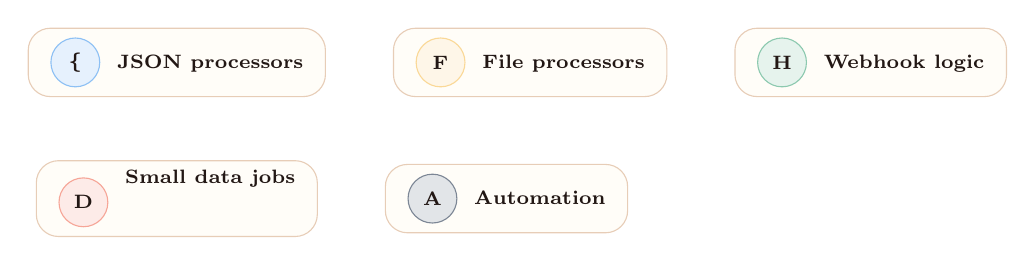
\begin{tikzpicture}[node distance=0.8cm and 0.85cm]
  \node[nodebox,minimum width=2.6cm] (json) {\circicon{Blue}{\{} JSON processors};
  \node[nodebox,minimum width=2.6cm,right=of json] (files) {\circicon{Gold}{F} File processors};
  \node[nodebox,minimum width=2.6cm,right=of files] (hooks) {\circicon{Green}{H} Webhook logic};
  \node[nodebox,minimum width=2.6cm,below=of json] (data) {\circicon{Coral}{D} Small data jobs};
  \node[nodebox,minimum width=2.6cm,right=of data] (auto) {\circicon{Navy}{A} Automation};
\end{tikzpicture}
\vspace{0.5cm}

{\large The prototype targets small Python services and short jobs.}
\end{contentframe}

\begin{contentframe}{Function code}
\begin{columns}[T,totalwidth=\linewidth]
\begin{column}{0.58\linewidth}
\begin{lstlisting}[language=Python]
def main(event, context):
    name = event.get("name", "world")
    print(f"hello {name}")
    return {"message": f"Hello, {name}!"}
\end{lstlisting}
\end{column}
\begin{column}{0.36\linewidth}
\Large
\plainitem{\texttt{event} carries input}\par\vspace{0.35cm}
\plainitem{\texttt{context} carries metadata}\par\vspace{0.35cm}
\plainitem{return value becomes result JSON}
\end{column}
\end{columns}
\end{contentframe}

\begin{contentframe}{Dependencies}
\centering
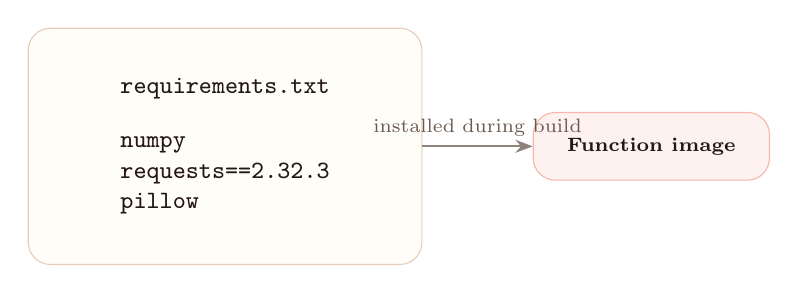
\begin{tikzpicture}
  \node[nodebox,minimum width=5.0cm,minimum height=3.0cm,align=left,font=\ttfamily\small] (req) {
    requirements.txt\\[0.3cm]
    numpy\\
    requests==2.32.3\\
    pillow
  };
  \node[actionbox,minimum width=3.0cm,right=1.4cm of req] (image) {Function image};
  \draw[line] (req) -- node[above,font=\scriptsize\color{Muted}]{installed during build} (image);
\end{tikzpicture}
\end{contentframe}

\begin{contentframe}{Function contract}
\begin{columns}[T,totalwidth=\linewidth]
  \begin{column}{0.47\linewidth}
    \Large
    \plainitem{Access mode}\par\vspace{0.28cm}
    \plainitem{Input file rules}\par\vspace{0.28cm}
    \plainitem{Expected output names}
  \end{column}
  \begin{column}{0.47\linewidth}
    \Large
    \plainitem{Memory limit}\par\vspace{0.28cm}
    \plainitem{Function timeout}\par\vspace{0.28cm}
    \plainitem{Output size limits}
  \end{column}
\end{columns}
\vspace{0.55cm}
{\large The contract gives users a predictable API and gives workers boundaries.}
\end{contentframe}

\begin{contentframe}{Access modes}
\centering
\renewcommand{\arraystretch}{1.45}
\begin{tabular}{>{\bfseries}p{0.24\linewidth}p{0.58\linewidth}}
\toprule
Private & owner or admin JWT required \\
Token & caller sends a function invocation token \\
Public & caller can invoke without auth \\
\bottomrule
\end{tabular}
\vspace{0.55cm}

{\large Invocation tokens stay separate from login JWTs.}
\end{contentframe}

\begin{contentframe}{Synchronous invocation}
\begin{columns}[T,totalwidth=\linewidth]
\begin{column}{0.48\linewidth}
\Large
\plainitem{JSON-only functions}\par\vspace{0.3cm}
\plainitem{No input files}\par\vspace{0.3cm}
\plainitem{No declared output files}\par\vspace{0.3cm}
\plainitem{Direct result when fast enough}
\end{column}
\begin{column}{0.46\linewidth}
\begin{lstlisting}[language={},basicstyle=\ttfamily\small]
POST /api/functions/4/invoke-sync/

{"name": "Ada"}

200 OK
{"message": "Hello, Ada!"}
\end{lstlisting}
\end{column}
\end{columns}
\end{contentframe}

\begin{contentframe}{Asynchronous invocation}
\begin{columns}[T,totalwidth=\linewidth]
\begin{column}{0.48\linewidth}
\Large
\plainitem{Durable job path}\par\vspace{0.3cm}
\plainitem{Supports files}\par\vspace{0.3cm}
\plainitem{Supports polling}\par\vspace{0.3cm}
\plainitem{Supports ZIP download}
\end{column}
\begin{column}{0.46\linewidth}
\begin{lstlisting}[language={},basicstyle=\ttfamily\small]
202 Accepted
{
  "invocation_id": 9274,
  "status": "queued",
  "read_token": "inv_..."
}
\end{lstlisting}
\end{column}
\end{columns}
\end{contentframe}

\begin{contentframe}{Result view}
\centering
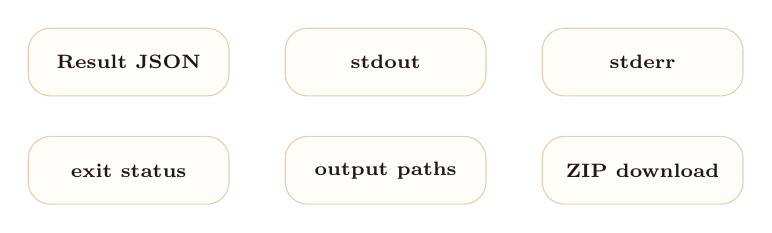
\begin{tikzpicture}[node distance=0.5cm and 0.7cm]
  \node[nodebox,minimum width=2.55cm] (r) {Result JSON};
  \node[nodebox,minimum width=2.55cm,right=of r] (out) {stdout};
  \node[nodebox,minimum width=2.55cm,right=of out] (err) {stderr};
  \node[nodebox,minimum width=2.55cm,below=of r] (exit) {exit status};
  \node[nodebox,minimum width=2.55cm,right=of exit] (files) {output paths};
  \node[nodebox,minimum width=2.55cm,right=of files] (zip) {ZIP download};
\end{tikzpicture}
\vspace{0.6cm}

{\large Simple responses stay small. Advanced responses expose diagnostics.}
\end{contentframe}

\begin{contentframe}{Frontend workflow}
\centering
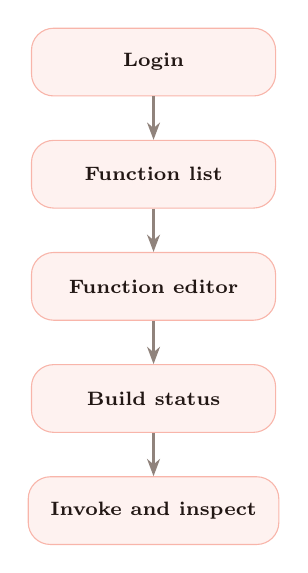
\begin{tikzpicture}[node distance=0.55cm]
  \node[actionbox,minimum width=3.1cm] (login) {Login};
  \node[actionbox,minimum width=3.1cm,below=of login] (list) {Function list};
  \node[actionbox,minimum width=3.1cm,below=of list] (edit) {Function editor};
  \node[actionbox,minimum width=3.1cm,below=of edit] (build) {Build status};
  \node[actionbox,minimum width=3.1cm,below=of build] (invoke) {Invoke and inspect};
  \draw[line] (login) -- (list);
  \draw[line] (list) -- (edit);
  \draw[line] (edit) -- (build);
  \draw[line] (build) -- (invoke);
\end{tikzpicture}
\end{contentframe}

\begin{contentframe}{Main services}
\centering
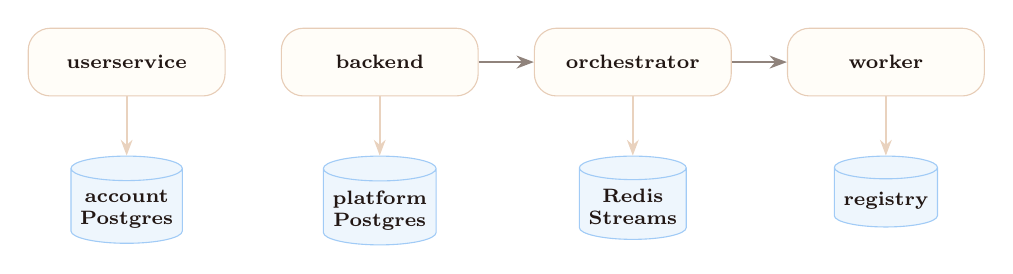
\begin{tikzpicture}[node distance=0.8cm and 0.7cm]
  \node[nodebox,minimum width=2.5cm] (user) {userservice};
  \node[nodebox,minimum width=2.5cm,right=of user] (backend) {backend};
  \node[nodebox,minimum width=2.5cm,right=of backend] (orch) {orchestrator};
  \node[nodebox,minimum width=2.5cm,right=of orch] (worker) {worker};
  \node[storebox,below=0.75cm of user] (upg) {account\\Postgres};
  \node[storebox,below=0.75cm of backend] (pg) {platform\\Postgres};
  \node[storebox,below=0.75cm of orch] (redis) {Redis\\Streams};
  \node[storebox,below=0.75cm of worker] (reg) {registry};
  \draw[softline] (user) -- (upg);
  \draw[softline] (backend) -- (pg);
  \draw[softline] (orch) -- (redis);
  \draw[softline] (worker) -- (reg);
  \draw[line] (backend) -- (orch);
  \draw[line] (orch) -- (worker);
\end{tikzpicture}
\end{contentframe}

\begin{contentframe}{Current deployment}
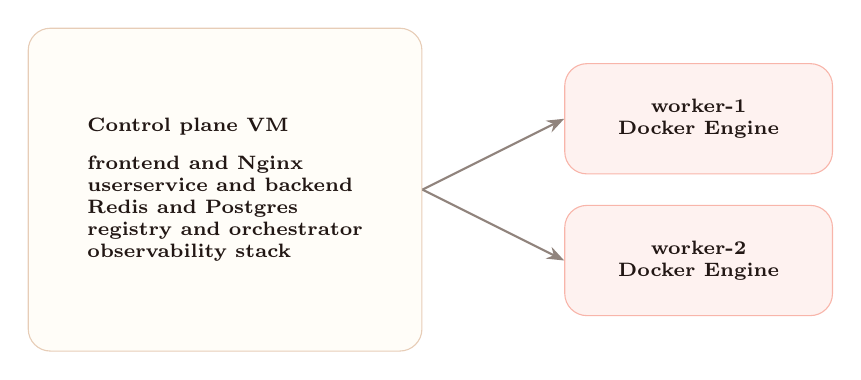
\begin{tikzpicture}[node distance=0.7cm]
  \node[nodebox,minimum width=5.0cm,minimum height=4.1cm,align=left] (cp) at (0,0) {
    \textbf{Control plane VM}\\[0.2cm]
    frontend and Nginx\\
    userservice and backend\\
    Redis and Postgres\\
    registry and orchestrator\\
    observability stack
  };
  \node[actionbox,minimum width=3.4cm,minimum height=1.4cm,right=1.8cm of cp,yshift=0.9cm] (w1) {worker-1\\Docker Engine};
  \node[actionbox,minimum width=3.4cm,minimum height=1.4cm,right=1.8cm of cp,yshift=-0.9cm] (w2) {worker-2\\Docker Engine};
  \draw[line] (cp.east) -- (w1.west);
  \draw[line] (cp.east) -- (w2.west);
\end{tikzpicture}
\end{contentframe}

\begin{contentframe}{Build flow}
\centering
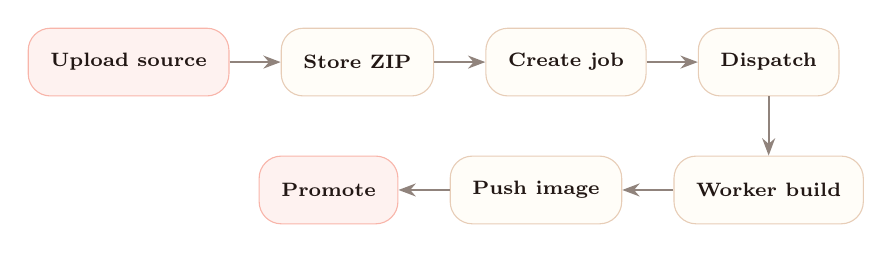
\begin{tikzpicture}[node distance=0.65cm]
  \node[actionbox] (a) {Upload source};
  \node[nodebox,right=of a] (b) {Store ZIP};
  \node[nodebox,right=of b] (c) {Create job};
  \node[nodebox,right=of c] (d) {Dispatch};
  \node[nodebox,below=0.75cm of d] (e) {Worker build};
  \node[nodebox,left=of e] (f) {Push image};
  \node[actionbox,left=of f] (g) {Promote};
  \draw[line] (a) -- (b);
  \draw[line] (b) -- (c);
  \draw[line] (c) -- (d);
  \draw[line] (d) -- (e);
  \draw[line] (e) -- (f);
  \draw[line] (f) -- (g);
\end{tikzpicture}
\end{contentframe}

\begin{contentframe}{Safe rebuilds}
\centering

\begin{tikzpicture}[node distance=1.0cm]
  \node[nodebox,minimum width=3.0cm] (old) {Active image};
  \node[actionbox,minimum width=3.0cm,right=of old] (cand) {Candidate image};
  \node[nodebox,minimum width=3.0cm,right=of cand] (next) {New active image};
  \draw[line] (old) -- node[above,font=\scriptsize\color{Muted}]{kept live} (cand);
  \draw[line] (cand) -- node[above,font=\scriptsize\color{Muted}]{only if build succeeds} (next);
\end{tikzpicture}
\vspace{0.65cm}

{\large Failed builds do not break the currently callable function.}
\end{contentframe}

\begin{contentframe}{Invocation flow}
\centering
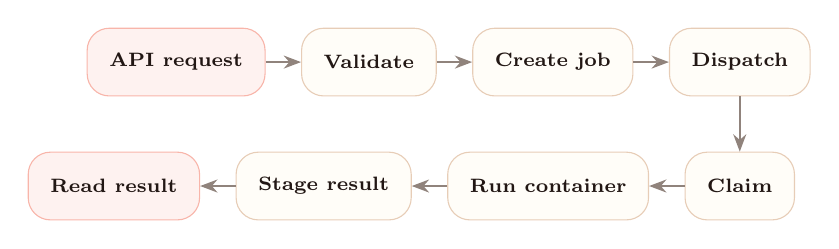
\begin{tikzpicture}[node distance=0.55cm and 0.45cm]
  \node[actionbox] (a) {API request};
  \node[nodebox,right=of a] (b) {Validate};
  \node[nodebox,right=of b] (c) {Create job};
  \node[nodebox,right=of c] (d) {Dispatch};
  \node[nodebox,below=0.7cm of d] (e) {Claim};
  \node[nodebox,left=of e] (f) {Run container};
  \node[nodebox,left=of f] (g) {Stage result};
  \node[actionbox,left=of g] (h) {Read result};
  \draw[line] (a) -- (b);
  \draw[line] (b) -- (c);
  \draw[line] (c) -- (d);
  \draw[line] (d) -- (e);
  \draw[line] (e) -- (f);
  \draw[line] (f) -- (g);
  \draw[line] (g) -- (h);
\end{tikzpicture}
\end{contentframe}

\begin{contentframe}{Files}
\Large
\plainitem{Input files are validated before execution}\par\vspace{0.35cm}
\plainitem{Output filenames must be declared during setup}\par\vspace{0.35cm}
\plainitem{Unexpected output files are rejected}\par\vspace{0.35cm}
\plainitem{Inputs, outputs, and logs expire with the invocation}
\end{contentframe}

\begin{contentframe}{Staged artifacts}
\begin{columns}[T,totalwidth=\linewidth]
\begin{column}{0.47\linewidth}
\smalllabel{Problem}
\Large A file can upload before the job is finalized.
\end{column}
\begin{column}{0.47\linewidth}
\smalllabel{Solution}
\Large Hide staged files until the finalizer commits them.
\end{column}
\end{columns}
\vspace{0.65cm}
\centering
\statuspill{Gold}{STAGED} \hspace{0.45cm}
\statuspill{Green}{COMMITTED} \hspace{0.45cm}
\statuspill{Blue}{VISIBLE}
\end{contentframe}

\begin{contentframe}{Orchestrator role}
\centering
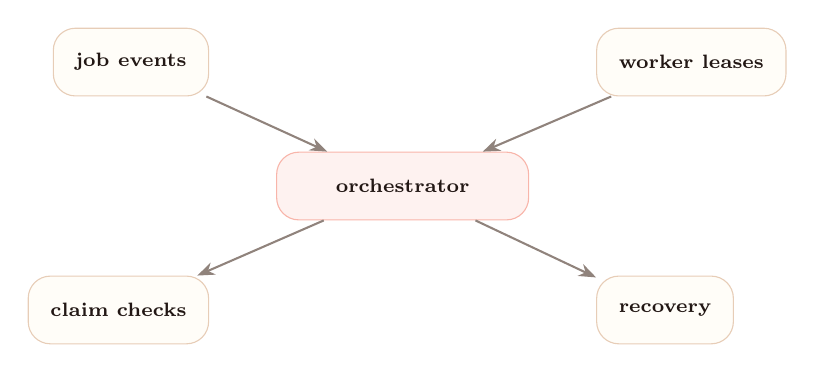
\begin{tikzpicture}[node distance=0.7cm and 0.85cm]
  \node[actionbox,minimum width=3.2cm] (orch) {orchestrator};
  \node[nodebox,above left=of orch] (events) {job events};
  \node[nodebox,above right=of orch] (workers) {worker leases};
  \node[nodebox,below left=of orch] (claims) {claim checks};
  \node[nodebox,below right=of orch] (recovery) {recovery};
  \draw[line] (events) -- (orch);
  \draw[line] (workers) -- (orch);
  \draw[line] (orch) -- (claims);
  \draw[line] (orch) -- (recovery);
\end{tikzpicture}
\vspace{0.4cm}

{\large The orchestrator owns active V2 job state in Redis.}
\end{contentframe}

\begin{contentframe}{Worker role}
\Large
\plainitem{Read assigned Redis Stream}\par\vspace{0.25cm}
\plainitem{Claim job through the orchestrator}\par\vspace{0.25cm}
\plainitem{Download source or inputs from backend}\par\vspace{0.25cm}
\plainitem{Run Docker build or function execution}\par\vspace{0.25cm}
\plainitem{Report completion and maintain warm containers}
\end{contentframe}

\begin{contentframe}{Reliability model}
\centering
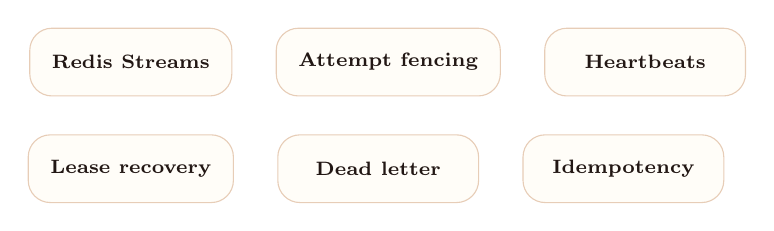
\begin{tikzpicture}[node distance=0.48cm and 0.55cm]
  \node[nodebox,minimum width=2.55cm] (streams) {Redis Streams};
  \node[nodebox,minimum width=2.55cm,right=of streams] (attempt) {Attempt fencing};
  \node[nodebox,minimum width=2.55cm,right=of attempt] (hb) {Heartbeats};
  \node[nodebox,minimum width=2.55cm,below=of streams] (lease) {Lease recovery};
  \node[nodebox,minimum width=2.55cm,right=of lease] (dlq) {Dead letter};
  \node[nodebox,minimum width=2.55cm,right=of dlq] (idem) {Idempotency};
\end{tikzpicture}
\vspace{0.55cm}

{\large Jobs either finish, recover, or move to a terminal failure state.}
\end{contentframe}

\begin{contentframe}{Warm containers}
\centering

\begin{tikzpicture}[node distance=1.0cm]
  \node[nodebox,minimum width=3.2cm] (cold) {Cold path\\create and start};
  \node[actionbox,minimum width=3.2cm,right=of cold] (warm) {Warm path\\reuse idle};
  \node[nodebox,minimum width=3.2cm,right=of warm] (runner) {Resident runner\\avoid startup};
  \draw[line] (cold) -- (warm);
  \draw[line] (warm) -- (runner);
\end{tikzpicture}
\vspace{0.7cm}

\bigstat{3918 ms}{old warm no-op median}\hspace{0.4cm}
\bigstat{88 ms}{resident runner no-op median}
\end{contentframe}

\begin{contentframe}{Performance bottlenecks}
\Large
\plainitem{Docker container create and start}\par\vspace{0.3cm}
\plainitem{Python module imports}\par\vspace{0.3cm}
\plainitem{File copying and output handling}\par\vspace{0.3cm}
\plainitem{Docker contention during concurrent bursts}
\end{contentframe}

\begin{contentframe}{Observability}
\centering
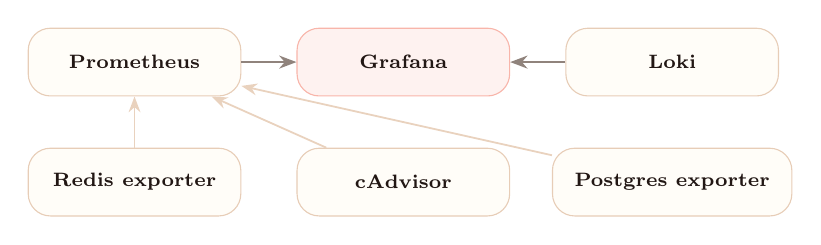
\begin{tikzpicture}[node distance=0.65cm and 0.7cm]
  \node[actionbox,minimum width=2.7cm] (grafana) {Grafana};
  \node[nodebox,minimum width=2.7cm,left=of grafana] (prom) {Prometheus};
  \node[nodebox,minimum width=2.7cm,right=of grafana] (loki) {Loki};
  \node[nodebox,minimum width=2.7cm,below=of prom] (redis) {Redis exporter};
  \node[nodebox,minimum width=2.7cm,below=of grafana] (cad) {cAdvisor};
  \node[nodebox,minimum width=2.7cm,below=of loki] (pg) {Postgres exporter};
  \draw[line] (prom) -- (grafana);
  \draw[line] (loki) -- (grafana);
  \draw[softline] (redis) -- (prom);
  \draw[softline] (cad) -- (prom);
  \draw[softline] (pg) -- (prom);
\end{tikzpicture}
\end{contentframe}

\begin{contentframe}{Lessons from failures}
\Large
\plainitem{Backend-centered coordination became too heavy}\par\vspace{0.26cm}
\plainitem{Docker copy and export paths were expensive}\par\vspace{0.26cm}
\plainitem{Vite dev serving is weak for production}\par\vspace{0.26cm}
\plainitem{Worker health missed consume-loop failure}\par\vspace{0.26cm}
\plainitem{Private registry refs broke after network changes}
\end{contentframe}

\begin{contentframe}{Current state}
\begin{columns}[T,totalwidth=\linewidth]
\begin{column}{0.48\linewidth}
\Large
\plainitem{Working frontend}\par\vspace{0.24cm}
\plainitem{Separate userservice}\par\vspace{0.24cm}
\plainitem{V2 orchestrator}\par\vspace{0.24cm}
\plainitem{Two distributed workers}
\end{column}
\begin{column}{0.48\linewidth}
\Large
\plainitem{Token invocation}\par\vspace{0.24cm}
\plainitem{Warm containers}\par\vspace{0.24cm}
\plainitem{Artifact storage}\par\vspace{0.24cm}
\plainitem{OpenAPI docs}
\end{column}
\end{columns}
\end{contentframe}

\begin{frame}[plain]
\begin{tikzpicture}[remember picture,overlay]
  \fill[Paper] (current page.south west) rectangle (current page.north east);
  \node[anchor=east,opacity=0.9] at ([xshift=0.75cm]current page.east)
    {
\includegraphics[height=7.3cm]{assets/fleeting-circus-mascot.png}};
\end{tikzpicture}
\vspace{0.7cm}
\hspace{0.35cm}
\begin{minipage}{0.62\linewidth}
  \smalllabel{Next work}
  \decktitle{Reliability and production hardening}
  \vspace{0.45cm}
  {\Large
  \plainitem{Recover worker consume-loop failures}\par\vspace{0.22cm}
  \plainitem{Harden distributed networking}\par\vspace{0.22cm}
  \plainitem{Add stronger build resource limits}\par\vspace{0.22cm}
  \plainitem{Serve the frontend as static production files}\par\vspace{0.22cm}
  \plainitem{Run longer failure and load tests}
  }
\end{minipage}
\end{frame}

\end{document}
